    \subsection{発展難易度}\label{節：発展難易度}\label{節：大学過去問ベースのもの}
      ここでは,漸化式を場合の数,確率,整数,図形,積分,極限の問題に使う10題を扱う.
      まず何を数列として追うかを選び,元の条件から漸化式を立て,最後に元の問いへ戻そう.
      一般項を求めることだけが目的ではない. 求めたい量の性質に応じて,和,差,剰余,不変量にも注目する.
      問1から問9は大学入試問題の構造・発想を参考に,問いや誘導を本書向けに再構成した演習である.
      問10は著者の掲載問題を改稿したもので,完全順列の古典的題材を扱う.
      参考資料は各問の末尾に示す. 問5は数学IIIの置換積分・部分積分・断面積による体積計算を前提とする.

      \subsubsection{問題}\label{節：発展難易度：問題}\label{節：大学過去問ベースのもの：問題}
        \begin{enumerate}[label=\textbf{問\arabic*.},leftmargin=3.8em,format=\bookitemlink{practice-entrance}{problem}{answer}]
          % F1: 正方形上の確率移動と分布の収束
          \item 正方形の頂点を時計回りに$A,B,C,D$とする.点$P$は初め$A$にあり,1秒ごとに,その頂点にとどまる,時計回りに隣の頂点へ移る,反時計回りに隣の頂点へ移る,の3つの操作から1つを選ぶ.どの操作も選ばれる確率は$\dfrac13$であり,各回の選択は独立である.
                $n$秒後に$P$が$A,C$にいる確率をそれぞれ$p_n,q_n$,\,$B,D$のいずれかにいる確率を$r_n$とする.ただし,\,$n=0,1,2,\ldots$である.
                
                \smallskip
                \noindent (1)~$p_{n+1},q_{n+1}$を$p_n,q_n,r_n$で表せ.
                
                \smallskip
                \noindent (2)~$u_n=p_n+q_n$,\,$v_n=p_n-q_n$とおく.$u_n,v_n$の一般項を求め,各頂点にいる確率を求めよ.
                
                \smallskip
                \noindent (3)~各頂点にいる確率の$n\to\infty$における極限を求めよ.
                \par\smallskip{\small\textit{\href{https://www.u-tokyo.ac.jp/content/400263415.pdf}{東京大学2024年理科第3問の状態分類を参考に再構成}}}
          % F2: 奇数が続く条件と2の因子
          \item 正の整数$a_0$から,数列$\{a_n\}$を
                \[
                  a_{n+1}=\begin{cases}
                    \dfrac{a_n}{2}&(a_n\text{が偶数}),\\[3pt]
                    \dfrac{3a_n+1}{2}&(a_n\text{が奇数})
                  \end{cases}
                \]
                によって定める.
                
                \smallskip
                \noindent (1)~$a_0,a_1,\ldots,a_m$がすべて奇数であるとき,$a_j+1$を$a_0$と$j$で表せ.ただし,\,$0\le j\le m$とする.
                
                \smallskip
                \noindent (2)~正整数$m$に対し,$a_0,a_1,\ldots,a_m$がすべて奇数となるような$a_0$をすべて求め,その最小値を答えよ.
                
                \smallskip
                \noindent (3)~$a_0+1=2^s t$と表す.ただし,\,$s$は$0$以上の整数,$t$は正の奇数である.初項$a_0$から連続して現れる奇数項の個数を求めよ.
                \par\smallskip{\small\textit{\href{https://www.kyoto-u.ac.jp/ja/admissions/undergrad/past-eq}{京都大学2024年理系第4問の偶奇分岐を参考に再構成}}}
          % F3: 畳み込み和が一定になる数列
          \item 数列$\{c_n\}$を
                \[
                  c_0=1,\qquad
                  c_{n+1}=\frac{2n+1}{2n+2}c_n
                  \quad(n=0,1,2,\ldots)
                \]
                によって定め,
                \[
                  T_n=\sum_{k=0}^{n}c_kc_{n-k}
                \]
                とする.
                
                \smallskip
                \noindent (1)~$c_n$を階乗を用いて表せ.ただし,\,$0!=1$とする.
                
                \smallskip
                \noindent (2)~正整数$n$に対し,
                \[
                  nT_n=\sum_{j=0}^{n-1}(2j+1)c_jc_{n-1-j}
                \]
                を示せ.さらに,この等式を用いて$T_n$を求めよ.
                
                \smallskip
                \noindent (3)~正整数$n$に対し,
                \[
                  \sum_{k=0}^{n}\binom{2k}{k}
                     \binom{2n-2k}{n-k}=4^n
                \]
                が成り立つことを示せ.
                \par\smallskip{\small\textit{\href{https://www.osaka-u.ac.jp/ja/admissions/faculty/general/files/9o1vy3/@@download/file}{大阪大学2025年文系第2問の畳み込み構造を参考に再構成}}}
          % F4: 内分を繰り返す平行四辺形
          \item 平行四辺形$A_0B_0C_0D_0$の頂点を反時計回りに並べる.
                一定の実数$t$が$0<t<1$を満たすとする.
                四角形$A_nB_nC_nD_n$の各辺上に,
                \[
                 \begin{aligned}
                 A_nA_{n+1}:A_{n+1}B_n&=t:(1-t),\\
                 B_nB_{n+1}:B_{n+1}C_n&=t:(1-t),\\
                 C_nC_{n+1}:C_{n+1}D_n&=t:(1-t),\\
                 D_nD_{n+1}:D_{n+1}A_n&=t:(1-t)
                 \end{aligned}
                \]
                となる点を取り,この操作を繰り返す.\,$n$は$0$以上の整数とする.
                \par\noindent
                (1) 各四角形は平行四辺形であり,対角線の交点が変わらないことを示せ.
                \par\noindent
                (2) $A_nB_nC_nD_n$の面積を$S_n$とする.\,$S_n$を$S_0,t,n$で表せ.
                \par\noindent
                (3) $n\to\infty$のとき,すべての頂点が最初の対角線の交点$O$に近づくことを示せ.
                \par\noindent
                (4) 初めの図形が辺長$\ell$の正方形で,\,$t=1/2$の場合を考える.
                操作を$n$回行った正方形の辺長を求めよ.
                また,有向線分$A_nB_n$の向きは,最初の向きからどれだけ回転するか.
                \par\smallskip{\small\textit{\href{https://www.densu.jp/tsukuba/22tsukubaspass.pdf}{筑波大学2022前期 第3問の内分操作を参考に独自に再構成}}}
          % F5: 積分を数列にして円錐を切る
          \item この問題では,数学IIIの部分積分・置換積分と,断面積による体積計算を用いる.
                正整数$n$に対して,
                \[
                 I_n=\int_0^{\pi/3}\frac{d\theta}{\cos^n\theta}
                \]
                とする.
                \par\noindent
                (1) $I_1,I_2$を求めよ.
                \par\noindent
                (2) $n\geq3$について$\,I_n$と$I_{n-2}$の関係式を求め,\,$I_3$を計算せよ.
                \par\noindent
                (3) 座標空間において,原点を頂点とし,平面$z=2$上の半径$2$の円を底面とする円錐を考える.
                その内部と表面は,
                \[
                 0\leq z\leq2,\qquad x^2+y^2\leq z^2
                \]
                で表される.この円錐のうち$x\geq1$を満たす部分の体積を求めよ.
                \par\smallskip{\small\textit{\href{https://www.nagoya-u.ac.jp/admissions/exam/upload/06_h31_sugakurikakei-seikai.pdf}{名古屋大学2019理系 第1問の構造を参考に独自に再構成}}}
          % F6: 一般項を求めずに減衰の速さを決める
          \item $\displaystyle a_1=1,\qquad
                a_{n+1}=\frac{a_n}{(1+2a_n)^2}$
                で数列$\{a_n\}$を定め,$b_n=1/a_n$とする.
                \par\noindent
                (1) すべての項が正であることを確かめ,$n\geq2$について$b_n>4n-3$を示せ.
                \par\noindent
                (2) 次の極限を求めよ.
                \[
                 \lim_{n\to\infty}\frac1n\sum_{k=1}^n a_k
                \]
                (3) $\displaystyle\lim_{n\to\infty}na_n$を求めよ.
                \par\smallskip{\small\textit{\href{https://toudainyuushi.com/wp-content/uploads/2020/06/2006S.pdf}{東京大学2006理科 第5問を参考に再構成した既存題を維持・増補}}}
          % F7: 1往復で整列できる札の配置
          \item $n$枚の札には$1,2,\ldots,n$の数字が1つずつ書かれている.
                これらを横一列に並べ, 隣り合う2枚を左から順に調べる.
                左の数字が右の数字より大きいときだけ交換し, 右端まで進む.
                続いて, 隣り合う2枚を右から順に調べ, 同じ規則で交換して左端まで戻る.
                この1往復で$1,2,\ldots,n$の順になる初期配置を\textbf{成功配置}と呼び, その個数を$c_n$とする.
                ただし,\,$n=1$では操作を行わず,\,$c_1=1$とする. 以下の問に答えよ.
                
                \smallskip
                \noindent (1)~$c_2,c_3$を求めよ. また,\,$n\ge2$として成功配置の最初の2枚の数字を$A_1,A_2$とするとき,
                少なくとも一方が$2$以下であることを示せ.
                
                \smallskip
                \noindent (2)~$n\ge3$とする. 最初の2枚に$1$を含む場合と,\,$1$を含まず$2$を含む場合に分けて数え,
                $c_n,c_{n-1},c_{n-2}$の関係式を求めよ.
                後者では, 最初の比較を済ませてから$2$の札を取り除くことを考えてよい.
                
                \smallskip
                \noindent (3)~$c_n$を求めよ.
                \par\smallskip{\small\textit{\href{https://www.u-tokyo.ac.jp/content/400239118.pdf}{東京大学2025年度理科第5問を参考に再構成}}}
          % F8: 巨大な項の整除と, 添字の互除法
          \item $\displaystyle a_1=1,\quad a_{n+1}=a_n^2+1$
                で定まる数列$\{a_n\}$について, 以下の問に答えよ.
                整数$x,y$の最大公約数を$\gcd(x,y)$と表す.
                
                \smallskip
                \noindent (1)~$a_n$が$5$の倍数となる正整数$n$をすべて求めよ.
                
                \smallskip
                \noindent (2)~任意の正整数$m,n$に対して,\,$a_m$が$a_n$を割り切ることと,
                $m$が$n$を割り切ることは同値であることを示せ.
                必要なら, 補助的に$a_0=0$と定めてよい.
                
                \smallskip
                \noindent (3)~任意の正整数$m,n$について
                \[
                 \gcd(a_m,a_n)=a_{\gcd(m,n)}
                \]
                が成り立つことを示し,\,$\gcd(a_{2026},a_{3040})$を求めよ.
                \par\smallskip{\small\textit{\href{https://www.densu.jp/tokyo/22tokyospass.pdf}{東京大学2022年度理科第2問を参考に再構成}}}
          % F9: 整数方程式の解を生み出す漸化式
          \item 正の整数$x,y,z$についての方程式
                \[
                 x^2+y^2+z^2=xyz
                \]
                を考える. 以下の問に答えよ.
                
                \smallskip
                \noindent (1)~$x=3$を満たす解$(3,y,z)$について,\,$y\le z$ならば
                $(3,z,3z-y)$も正の整数解であり,\,$3z-y>z$となることを示せ.
                
                \smallskip
                \noindent (2)~数列$\{u_n\}$を
                \[
                 u_0=u_1=3,\qquad
                 u_{n+2}=3u_{n+1}-u_n\quad(n\ge0)
                \]
                によって定める. 一般項を求めよ.
                
                \smallskip
                \noindent (3)~$(3,u_n,u_{n+1})$がすべての$n\ge0$について上の方程式の正の整数解となることを示せ.
                さらに, 異なる正の整数解が無限個あることを示し,
                $\displaystyle\lim_{n\to\infty}u_{n+1}/u_n$を求めよ.
                \par\smallskip{\small\textit{\href{https://toudainyuushi.com/wp-content/uploads/2020/06/2006S.pdf}{東京大学2006年度理科第4問を参考に独自に作成}}}
          % F10: 元のペアをすべて解消する組み替え
          \item $n$を正の整数とする. 互いに異なる$2n$個の要素
                \[
                 A_1,\ldots,A_n,\quad B_1,\ldots,B_n
                \]
                があり, 初めは$A_i$と$B_i$がペアを組んでいる.
                各ペアを$A$側と$B$側から1個ずつ選んで作り, すべての要素をちょうど1回ずつ使って$n$組のペアを作り直す.
                完成した組合せを数え, ペアを並べる順序や組み替える操作の手順は区別しない.
                元のペア$(A_i,B_i)$が1組も残らない組合せの数を$S(n)$とする.
                以下,\,$S(0)=1$と定める.
                \par\smallskip
                (1) $S(1),S(2),S(3)$を求めよ.
                \par\smallskip
                (2) $A_1$の相手を$B_j$とする.
                $A_j$の相手が$B_1$である場合と, そうでない場合に分け,
                $S(n),S(n-1),S(n-2)$の関係式を求めよ.
                \par\smallskip
                (3) $S(n)-nS(n-1)$を求め,\,$S(n)$を有限和で表せ.
                \par\smallskip
                (4) $r$を$0\le r\le n$を満たす整数とする.
                元のペアがちょうど$r$組残る組合せの数を求めよ.
                また, 全$n!$通りの組合せについて, 元のペアが残る組数の平均値を求めよ.
                \par\smallskip{\small\textit{\href{https://jukenmath.net/problems/798}{著者作問「ペアの入れ替えパターン数」}}}
        \end{enumerate}

      \subsubsection{方針}\label{節：発展難易度：方針}\label{節：大学過去問ベースのもの：方針}
        \begin{enumerate}[label=\textbf{問\arabic*.},leftmargin=3.8em,format=\bookitemlink{practice-entrance}{hint}{problem}]
          % F1: 正方形上の確率移動と分布の収束
          \item $A$への移動は,$A$にとどまる場合と,$B,D$から移る場合に分かれる.$p_n+q_n+r_n=1$を使って和の式から$r_n$を消去する.差の式では$r_n$が相殺する.$B,D$にいる確率が等しいことも,操作の対称性から確かめる.
          % F2: 奇数が続く条件と2の因子
          \item 奇数の分岐だけを使える間は,$a_{n+1}+1=\dfrac32(a_n+1)$となる.(2)では,$a_m+1$が偶数になる必要条件を求めた後,その条件から実際に各項が奇数になることを確認する.(3)では,$a_j+1$から2の因子が1つずつ減ることに注目する.
          % F3: 畳み込み和が一定になる数列
          \item (1)は階比型として係数を掛ける.(2)では,$n=k+(n-k)$と分け,\,$k$を$n-k$に入れ替えて同じ和が現れることを使う.漸化式で$kc_k$を$c_{k-1}$に直した後も,添字を逆順にした2つの式を加えると係数が一定になる.(3)は(1)の式を$T_n$に代入する.
          % F4: 内分を繰り返す平行四辺形
          \item 隣接する辺を$\boldsymbol p_n=\overrightarrow{A_nB_n}$,
                \,$\boldsymbol q_n=\overrightarrow{A_nD_n}$とする.
                面積は,内側の四角形の周囲に残る四つの三角形を引けばよい.
                収束を示すときは,\,$|\boldsymbol p_n|^2+|\boldsymbol q_n|^2$の漸化式を作る.
                正方形の場合は,辺を表す複素数への掛け算で回転を読み取る.
          % F5: 積分を数列にして円錐を切る
          \item $I_n$を$\cos^{-(n-2)}\theta$と$\cos^{-2}\theta$の積として部分積分し,
                $\sin^2\theta=1-\cos^2\theta$で整理する.
                体積は平面$z=$一定で切る.断面は半径$z$の円の弓形になるので,
                弓形の半分の中心角を$\theta$とし,$z\cos\theta=1$で置換する.
          % F6: 一般項を求めずに減衰の速さを決める
          \item 逆数を取ると,$b_{n+1}-b_n=4+4a_n$になる.
                階差を足し合わせた式を使い,まず$a_n\to0$を示す.
                平均の極限は,有限個の初期項と,十分小さくなった残りの項に分けて評価する.
                最後に$b_n/n$を調べ,$na_n$へ戻す.
          % F7: 1往復で整列できる札の配置
          \item 最初の比較の後, 左端には$\min(A_1,A_2)$が残る. この札がその後で触れられるのは, 復路の最後の比較だけである.
                個数を数える際には, 最初の2枚のどちらに$1$または$2$があるかで4つに分ける.
                $1$を取り除く場合と$2$を取り除く場合は, 小さい配置との対応が異なることに注意する.
          % F8: 巨大な項の整除と, 添字の互除法
          \item (1)では項そのものを計算する代わりに,\,$5$で割った余りに漸化式を適用する.
                (2)では法を$a_m$へ変える. $a_0=0$とおけば,\,$a_m$から先の余りは$a_0$からの余りを繰り返す.
                (3)では$n$を$m$で割った余りへ置き換える操作が, 項の最大公約数を変えないことを示す.
          % F9: 整数方程式の解を生み出す漸化式
          \item (1)では$9+z^2+(3z-y)^2-3z(3z-y)$を整理する.
                この整理で保たれる式を,\,(3)では隣接する2項に適用する.
                (2)は実数解型の3項間漸化式である. (3)の整数性は一般項を展開するよりも, 初期値と漸化式から示す方が短い.
          % F10: 元のペアをすべて解消する組み替え
          \item (2) 後者では,\,$B_1$の相手を$A_k$とする.
                $A_1,B_1$を除き,\,$A_k$と$B_j$をペアにして,\,$n-1$組の問題との対応を考える.
                (3) 3項間の関係式を,\,$S(n)-nS(n-1)$について書き直す.
                その後,\,$n!$で割って階差を作る.
                (4) 残すペアを選んでから, 残りを完全に組み替える.
                平均値は, 各元のペアが何通りの組合せに含まれるかを数えると短い.
        \end{enumerate}

      \subsubsection{解答}\label{節：発展難易度：解答}\label{節：大学過去問ベースのもの：解答}
        \begin{enumerate}[label=\textbf{問\arabic*.},leftmargin=3.8em,format=\bookitemlink{practice-entrance}{answer}{problem}]
          % F1: 正方形上の確率移動と分布の収束
          \item (1)~
                \[
                  p_{n+1}=\frac{p_n+r_n}{3},\qquad
                  q_{n+1}=\frac{q_n+r_n}{3}.
                \]
                (2)~
                \[
                \begin{aligned}
                  u_n&=\frac12+\frac12\left(-\frac13\right)^n,\\
                  v_n&=\left(\frac13\right)^n.
                \end{aligned}
                \]
                したがって
                \[
                \begin{aligned}
                  p_n&=\frac14+\frac12\left(\frac13\right)^n
                       +\frac14\left(-\frac13\right)^n,\\
                  q_n&=\frac14-\frac12\left(\frac13\right)^n
                       +\frac14\left(-\frac13\right)^n.
                \end{aligned}
                \]
                $B,D$にいる確率はそれぞれ
                \[
                  \frac14-\frac14\left(-\frac13\right)^n
                \]
                である.(3)~極限はいずれも$\dfrac14$である.
          % F2: 奇数が続く条件と2の因子
          \item (1)~
                \[
                  a_j+1=\frac{3^j}{2^j}(a_0+1)
                  \quad(0\le j\le m).
                \]
                (2)~求める初期値は
                \[
                  a_0=2^{m+1}\ell-1
                  \quad(\ell=1,2,3,\ldots)
                \]
                であり,最小値は$2^{m+1}-1$である.
                
                (3)~奇数項の個数は$s$である.$s\ge1$のとき,$a_0,\ldots,a_{s-1}$が奇数であり,$a_s=3^s t-1$は偶数である.$s=0$のときは初項から偶数である.
          % F3: 畳み込み和が一定になる数列
          \item (1)~
                \[
                  c_n=\frac{(2n)!}{4^n(n!)^2}
                     =\frac1{4^n}\binom{2n}{n}.
                \]
                (2)~設問の等式から$T_n=T_{n-1}$が得られ,$T_0=1$より
                \[
                  T_n=1\quad(n=0,1,2,\ldots).
                \]
                (3)~$c_kc_{n-k}$を(1)の式で表し,$T_n=1$の両辺を$4^n$倍すれば示される.
          % F4: 内分を繰り返す平行四辺形
          \item (1) 対角線の交点は常に$O$である.
                \par\noindent
                (2) $\rho=(1-t)^2+t^2$と置くと,
                \[
                 S_n=S_0\rho^n.
                \]
                (3) 四つの頂点はすべて$O$に近づく.
                \par\noindent
                (4) 辺長は$\ell\,2^{-n/2}$であり,有向線分の向きは反時計回りに$n\pi/4$だけ回転する.
                向きの角は$2\pi$の整数倍の違いを同一視する.
          % F5: 積分を数列にして円錐を切る
          \item (1)
                \[
                 I_1=\log(2+\sqrt3),\qquad I_2=\sqrt3.
                \]
                (2)
                \[
                 (n-1)I_n=(n-2)I_{n-2}+2^{n-2}\sqrt3,
                \]
                \[
                 I_3=\sqrt3+\frac12\log(2+\sqrt3).
                \]
                (3) 求める体積は
                \[
                 \frac{8\pi}{9}-\frac{4\sqrt3}{3}
                 +\frac13\log(2+\sqrt3).
                \]
                ここで$\log$は自然対数である.
          % F6: 一般項を求めずに減衰の速さを決める
          \item (1) すべての項は正であり,
                \[
                 b_n=4n-3+4\sum_{k=1}^{n-1}a_k>4n-3
                 \qquad(n\geq2).
                \]
                (2) 極限は$0$である.
                \par\noindent
                (3) 極限は$1/4$である.
          % F7: 1往復で整列できる札の配置
          \item (1)~$c_2=2,\ c_3=6$である.
                
                (2)~$n\ge3$に対して
                \[
                  c_n=4c_{n-1}-2c_{n-2}.
                \]
                (3)~したがって,
                \[
                  \boxed{\displaystyle
                  c_n=\frac{(2+\sqrt2)^{n-1}+(2-\sqrt2)^{n-1}}2}
                  \quad(n\ge1).
                \]
          % F8: 巨大な項の整除と, 添字の互除法
          \item (1)~$n=3,6,9,\ldots$, すなわち$3$の正の倍数である.
                
                (2)~$a_m\mid a_n\ \Longleftrightarrow\ m\mid n$である.
                
                (3)~$\gcd(a_m,a_n)=a_{\gcd(m,n)}$であり,
                \[
                 \boxed{\gcd(a_{2026},a_{3040})=a_2=2}.
                \]
          % F9: 整数方程式の解を生み出す漸化式
          \item $\displaystyle\alpha=\frac{3+\sqrt5}2,\quad
                \beta=\frac{3-\sqrt5}2$とおくと,
                \[
                 \boxed{\displaystyle
                 u_n=\frac32\left\{
                 \alpha^n+\beta^n-
                 \frac{\alpha^n-\beta^n}{\sqrt5}
                 \right\}}.
                \]
                $(3,u_n,u_{n+1})$は正の整数解であり,\,$n\ge1$で$u_{n+1}>u_n$だから異なる解が無限個得られる.
                また,
                \[
                 \boxed{\displaystyle
                 \lim_{n\to\infty}\frac{u_{n+1}}{u_n}
                 =\frac{3+\sqrt5}2}.
                \]
          % F10: 元のペアをすべて解消する組み替え
          \item (1)
                \[
                 S(1)=0,\quad S(2)=1,\quad S(3)=2.
                \]
                (2)
                \[
                 S(n)=(n-1)\{S(n-1)+S(n-2)\}
                 \quad(n\ge2).
                \]
                (3)
                \[
                 S(n)-nS(n-1)=(-1)^n,
                \]
                \[
                 \boxed{S(n)=n!\sum_{k=0}^{n}\frac{(-1)^k}{k!}}.
                \]
                (4) 組合せの数は
                \[
                 \binom{n}{r}S(n-r).
                \]
                元のペアが残る組数の平均値は$1$である.
        \end{enumerate}

      \subsubsection{解法}\label{節：発展難易度：解法}\label{節：大学過去問ベースのもの：解法}
        \begin{enumerate}[label=\textbf{問\arabic*.},leftmargin=3.8em,format=\bookitemlink{practice-entrance}{solution}{problem}]
          % F1: 正方形上の確率移動と分布の収束
          \item \textbf{(1)~直前の位置で場合を分ける.}
                $n+1$秒後に$A$にいるためには,$n$秒後に$A$にいてとどまるか,$B$にいて反時計回りに移るか,$D$にいて時計回りに移ればよい.これらは同時には起こらないから,確率を加えられる.
                $B,D$のどちらにいても,次に$A$へ移る確率は$\dfrac13$である.よって,その2頂点にいる確率の合計$r_n$を用いて
                \[
                  p_{n+1}=\frac13p_n+\frac13r_n
                \]
                と書ける.同様に
                \[
                  q_{n+1}=\frac13q_n+\frac13r_n
                \]
                である.状態をまとめてよい理由は,$B,D$から$A,C$への移動確率がそれぞれ同じだからである.
                
                \smallskip
                \textbf{(2)~和と差で連立を解く.}
                初めは$A$にいるので,
                \[
                  p_0=1,\quad q_0=0,\quad r_0=0.
                \]
                また,必ず4頂点のどれかにいるから
                \[
                  p_n+q_n+r_n=1.
                \]
                2本の漸化式を加え,$r_n=1-u_n$を代入すると
                \[
                \begin{aligned}
                  u_{n+1}&=\frac{u_n+2r_n}{3}\\
                         &=\frac23-\frac13u_n.
                \end{aligned}
                \]
                これは本編の特性方程式型である.定数の解$\dfrac12$を引くと
                \[
                  u_{n+1}-\frac12=-\frac13\left(u_n-\frac12\right).
                \]
                $u_0=1$より
                \[
                  u_n=\frac12+\frac12\left(-\frac13\right)^n.
                \]
                一方,2本の漸化式を引くと,$r_n$の項が消え,
                \[
                  v_{n+1}=\frac13v_n,\qquad v_0=1
                \]
                となる.したがって
                \[
                  v_n=\left(\frac13\right)^n.
                \]
                本編の連立漸化式で用いたように,和と差を選ぶことで,2本の数列を別々に解ける形にしている.
                $\displaystyle p_n=\frac{u_n+v_n}{2}$,\,$\displaystyle q_n=\frac{u_n-v_n}{2}$より,(2)の式を得る.
                
                $B,D$にいる確率は等しい.実際,時計回りと反時計回りをすべて入れ替えると,$A,C$を固定して$B,D$を交換する経路になる.もとの経路と確率は同じであり,この対応は逆向きにも戻せる.よって,それぞれの確率は
                \[
                  \frac{r_n}{2}=\frac{1-u_n}{2}
                  =\frac14-\frac14\left(-\frac13\right)^n
                \]
                となる.求めた4つの確率に$n=0$を代入すると,初期条件も満たす.
                
                \smallskip
                \textbf{(3)~出発点の影響が消える.}
                公比の絶対値がいずれも$\dfrac13<1$なので,
                \[
                  \left(\frac13\right)^n\to0,\qquad
                  \left(-\frac13\right)^n\to0.
                \]
                したがって,各頂点にいる確率はすべて$\dfrac14$に近づく.
                対称な図形であっても,初めは$A$に確率が集中している.その偏りが時間とともに消えることを,漸化式から示せたのである.また,$u_n-\dfrac12$は符号を交互に変える.対頂点の組$\{A,C\}$にいる確率は,$\dfrac12$の上下を行き来しながら近づく.
          % F2: 奇数が続く条件と2の因子
          \item \textbf{(1)~使われる分岐を固定する.}
                偶奇で式が変わるので,初めから1本の式で全項を求めようとすると難しい.ここでは,奇数が続く区間に限って考える.
                $a_j$が奇数である間は
                \[
                  a_{j+1}=\frac32a_j+\frac12.
                \]
                本編の特性方程式型と同じく,定数の解$-1$を引けば
                \[
                  a_{j+1}+1=\frac32(a_j+1)
                \]
                となる.したがって,等比数列の式から
                \[
                  a_j+1=\frac{3^j}{2^j}(a_0+1)
                  \quad(0\le j\le m)
                \]
                を得る.この式を使える範囲は,奇数の分岐が使われる範囲である.
                
                \smallskip
                \textbf{(2)~必要条件を求め,逆向きに確認する.}
                まず,$a_0,\ldots,a_m$がすべて奇数であると仮定する.(1)より
                \[
                  3^m(a_0+1)=2^m(a_m+1).
                \]
                $a_m+1$は偶数なので,右辺は$2^{m+1}$で割り切れる.$3^m$と$2^{m+1}$は互いに素だから,$a_0+1$も$2^{m+1}$で割り切れる.よって
                \[
                  a_0=2^{m+1}\ell-1
                  \quad(\ell\text{は正整数})
                \]
                が必要である.
                
                次に,この形の$a_0$から始めれば条件を満たすことを示す.
                \[
                  b_j=3^j2^{m+1-j}\ell-1
                  \quad(0\le j\le m)
                \]
                とおく.$m+1-j\ge1$なので,$b_j$はすべて正の奇数である.また,$b_0=a_0$であり,$0\le j<m$で
                \[
                \begin{aligned}
                  \frac{3b_j+1}{2}
                    &=3^{j+1}2^{m-j}\ell-1\\
                    &=b_{j+1}
                \end{aligned}
                \]
                が成立する.したがって,各段階で実際に奇数の分岐が使われ,$a_j=b_j$となる.これで十分性も示された.
                
                $\ell$が正整数であることから,最小の初期値は$\ell=1$のときの$2^{m+1}-1$である.単に仮定の下で式を求めるだけでなく,その式が仮定に矛盾しないことを逆向きに確かめる点が大切である.
                
                \smallskip
                \textbf{(3)~奇数区間の長さを決める.}
                $s=0$なら$a_0+1=t$は奇数であり,$a_0$は偶数なので答えは$0$である.
                $s\ge1$とする.$0\le j\le s$について
                \[
                  b_j=3^j2^{s-j}t-1
                \]
                とおく.$j<s$なら$2^{s-j}$は偶数だから,$b_j$は正の奇数である.先ほどと同じ計算で,これらの奇数の分岐から$b_{j+1}$が得られるので,$a_j=b_j$である.最後に
                \[
                  a_s=3^s t-1
                \]
                は偶数となる.よって,初項から続く奇数項は$a_0$から$a_{s-1}$までの$s$個である.
                
                例えば,$a_0=7$なら$a_0+1=2^3$なので,奇数項は3個続く.実際,
                \[
                  7,\ 11,\ 17,\ 26,\ldots
                \]
                となる.見た目には偶奇で複雑に分岐する数列でも,最初の奇数区間の長さは$a_0+1$に含まれる2の因子だけで決まる.
          % F3: 畳み込み和が一定になる数列
          \item \textbf{(1)~各項は階比型で求められる.}
                $n\ge1$に対し,係数を掛け合わせると
                \[
                  c_n=\prod_{j=0}^{n-1}\frac{2j+1}{2j+2}.
                \]
                分母は$2\cdot4\cdots2n=2^n n!$である.分子の奇数の積は,$(2n)!$から偶数の積を取り除いて
                \[
                  1\cdot3\cdots(2n-1)=\frac{(2n)!}{2^n n!}
                \]
                と表せる.よって
                \[
                  c_n=\frac{(2n)!}{4^n(n!)^2}.
                \]
                この式は$n=0$でも$c_0=1$を与える.
                
                \smallskip
                \textbf{(2)~求めたい和そのものを追う.}
                一般項は分かったが,これを直ちに$T_n$に代入すると,階乗を含む積の和になる.ここでは各項を展開するよりも,$T_n$と1つ前の$T_{n-1}$の関係を探す.
                まず,$n=k+(n-k)$を各項に掛けて
                \[
                \begin{aligned}
                  nT_n
                   &=\sum_{k=0}^{n}kc_kc_{n-k}\\
                   &\quad+\sum_{k=0}^{n}(n-k)c_kc_{n-k}.
                \end{aligned}
                \]
                第2の和は,添字を$\ell=n-k$に変えると
                \[
                  \sum_{\ell=0}^{n}\ell c_{n-\ell}c_\ell
                \]
                となり,第1の和と同じである.したがって
                \[
                  nT_n=2\sum_{k=1}^{n}kc_kc_{n-k}.
                \]
                ここで,$k=0$の項は$0$なので取り除いた.
                もとの漸化式を1つ前の添字で書くと
                \[
                  2kc_k=(2k-1)c_{k-1}\quad(k\ge1).
                \]
                これを使い,$j=k-1$に変えれば
                \[
                \begin{aligned}
                  nT_n
                   &=\sum_{k=1}^{n}(2k-1)c_{k-1}c_{n-k}\\
                   &=\sum_{j=0}^{n-1}(2j+1)c_jc_{n-1-j}
                \end{aligned}
                \]
                となり,設問の等式を得る.
                
                右辺を$U_n$とする.添字を$\ell=n-1-j$に入れ替えてから,再び$\ell$を$j$と書けば
                \[
                  U_n=\sum_{j=0}^{n-1}(2n-2j-1)c_jc_{n-1-j}.
                \]
                元の式とこの式を加えると,係数の和は
                \[
                  (2j+1)+(2n-2j-1)=2n
                \]
                となる.よって
                \[
                  2U_n=2n\sum_{j=0}^{n-1}c_jc_{n-1-j}
                        =2nT_{n-1}.
                \]
                したがって,$nT_n=U_n=nT_{n-1}$である.$n\ge1$なので$n$で割り,
                \[
                  T_n=T_{n-1}
                \]
                を得る.これは差が$0$の等差型と見ることができる.$T_0=c_0^2=1$より,すべての$n\ge0$で$T_n=1$である.
                
                一般項の代入より先に,求めたい量に漸化式を立てた.これは本編の総和型と同じく,和を1本の数列として扱う考え方である.この問題では,積の中の2つの添字の和が一定であることと,その添字を交換しても積が変わらないことが鍵になった.
                
                \smallskip
                \textbf{(3)~二項係数の恒等式へ戻す.}
                (1)より
                \[
                \begin{aligned}
                  c_kc_{n-k}
                    &=\frac1{4^k}\binom{2k}{k}
                      \frac1{4^{n-k}}\binom{2n-2k}{n-k}\\
                    &=\frac1{4^n}\binom{2k}{k}
                      \binom{2n-2k}{n-k}.
                \end{aligned}
                \]
                したがって,$T_n=1$の式を$4^n$倍すると,(3)の等式が得られる.
                例えば,$n=2$では
                \[
                  1\cdot6+2\cdot2+6\cdot1=16=4^2
                \]
                である.各$c_n$は複雑な階乗で表される一方,同じ添字の和をもつ積を集めると常に$1$になる.各項の姿からは見えにくい性質を,和の漸化式が明らかにしている.
          % F4: 内分を繰り返す平行四辺形
          \item 図形が変わるたびに四つの頂点を別々に追うと,計算が増える.
                平行四辺形を決める二本の辺と,図形の中心に注目する.
                \par\noindent
                \textbf{(1) 内分をベクトルの式にする.}
                位置ベクトルを$\boldsymbol a_n,\boldsymbol b_n,
                \boldsymbol c_n,\boldsymbol d_n$とする.
                内分の条件より,
                \[
                 \begin{aligned}
                 \boldsymbol a_{n+1}&=(1-t)\boldsymbol a_n+t\boldsymbol b_n,\\
                 \boldsymbol b_{n+1}&=(1-t)\boldsymbol b_n+t\boldsymbol c_n,\\
                 \boldsymbol c_{n+1}&=(1-t)\boldsymbol c_n+t\boldsymbol d_n,\\
                 \boldsymbol d_{n+1}&=(1-t)\boldsymbol d_n+t\boldsymbol a_n.
                 \end{aligned}
                \]
                いま,$A_nB_nC_nD_n$が平行四辺形で,中心の位置ベクトルが$\boldsymbol o$なら,
                \[
                 \boldsymbol a_n+\boldsymbol c_n
                 =\boldsymbol b_n+\boldsymbol d_n=2\boldsymbol o.
                \]
                したがって,
                \[
                 \begin{aligned}
                 \boldsymbol a_{n+1}+\boldsymbol c_{n+1}
                  &=(1-t)\,2\boldsymbol o+t\,2\boldsymbol o\\
                  &=2\boldsymbol o,
                 \end{aligned}
                \]
                同様に$\boldsymbol b_{n+1}+\boldsymbol d_{n+1}=2\boldsymbol o$である.
                二本の対角線は同じ点$O$で二等分されるので,次の図形も平行四辺形で,中心は変わらない.
                初めの図形は平行四辺形だから,この性質は数学的帰納法ですべての$n$について成り立つ.
                \par\noindent
                \textbf{(2) 面積を数列にする.}
                内側の四角形の周囲には四つの三角形が残る.
                たとえば頂点$A_n$にある三角形$A_nA_{n+1}D_{n+1}$では,
                二辺がそれぞれ$|A_nB_n|$の$t$倍と$|A_nD_n|$の$1-t$倍である.
                よって面積は$\frac12t(1-t)S_n$になる.
                ほかの三つも同じ面積なので,
                \[
                 \begin{aligned}
                 S_{n+1}
                 &=S_n-4\cdot\frac12t(1-t)S_n\\
                 &=\{(1-t)^2+t^2\}S_n.
                 \end{aligned}
                \]
                ここで初めて,図形の問いが本編の等比型になった.
                \,$\rho=(1-t)^2+t^2$と置けば,
                \[
                 S_n=S_0\rho^n.
                \]
                $\rho>0$なので面積は常に正であり,各平行四辺形は退化しない.
                \par\noindent
                \textbf{(3) 面積の収束だけで終えない.}
                面積が$0$に近づくだけでは,細長い図形になる可能性を除けない.
                そこで,二本の辺の長さも調べる.
                \[
                 \boldsymbol p_n=\boldsymbol b_n-\boldsymbol a_n,
                 \qquad
                 \boldsymbol q_n=\boldsymbol d_n-\boldsymbol a_n
                \]
                とすると,内分の式と平行四辺形の性質より,
                \[
                 \begin{cases}
                 \boldsymbol p_{n+1}=(1-t)\boldsymbol p_n+t\boldsymbol q_n,\\
                 \boldsymbol q_{n+1}=-t\boldsymbol p_n+(1-t)\boldsymbol q_n.
                 \end{cases}
                \]
                連立式から一つの数列を取り出すため,長さの二乗を足した
                \[
                 E_n=|\boldsymbol p_n|^2+|\boldsymbol q_n|^2
                \]
                を考える.内積の交差項が打ち消し合うので,
                \[
                 \begin{aligned}
                 E_{n+1}
                 &=|(1-t)\boldsymbol p_n+t\boldsymbol q_n|^2\\
                 &\quad+|-t\boldsymbol p_n+(1-t)\boldsymbol q_n|^2\\
                 &=\rho E_n.
                 \end{aligned}
                \]
                よって$E_n=\rho^nE_0$である.
                $0<t<1$より$0<\rho=1-2t(1-t)<1$である.
                二乗は非負だから,両方の辺の長さは$0$へ近づく.
                また,$O$は対角線の中点なので,
                \[
                 \overrightarrow{OA_n}=-\frac{\boldsymbol p_n+\boldsymbol q_n}{2},
                 \qquad
                 |OA_n|\leq\frac{|\boldsymbol p_n|+|\boldsymbol q_n|}{2}.
                \]
                右辺は$0$に近づく.ほかの頂点についても$\boldsymbol p_n,\boldsymbol q_n$の符号が変わるだけだから,
                同じ評価ができる.したがって四つの頂点はすべて$O$に近づく.
                \par\noindent
                \textbf{(4) 正方形では複素数の積になる.}
                正方形が反時計回りに並んでいるとき,$\boldsymbol q_n$は$\boldsymbol p_n$を反時計回りに$\pi/2$回転したものである.
                それぞれを表す複素数を$z_n,w_n$とすると,$w_n=iz_n$である.
                \,$t=1/2$を連立式に入れると,
                \[
                 z_{n+1}=\frac{1+i}{2}z_n,
                 \qquad
                 w_{n+1}=iz_{n+1}.
                \]
                したがって次も正方形であり,
                \[
                 z_n=\left(\frac{1+i}{2}\right)^n z_0.
                \]
                ここで,
                \[
                 \frac{1+i}{2}
                 =\frac1{\sqrt2}\left(\cos\frac\pi4+i\sin\frac\pi4\right).
                \]
                ド・モアブルの定理より,
                \[
                 z_n=2^{-n/2}
                 \left(\cos\frac{n\pi}{4}+i\sin\frac{n\pi}{4}\right)z_0.
                \]
                よって辺長は$\ell\,2^{-n/2}$,有向線分の回転角は反時計回りに$n\pi/4$である.
                \par
                正方形では内分という操作が,中心を固定した回転と縮小そのものになる.
                一般の平行四辺形については,二本の辺を混ぜる連立式と面積の等比性が成り立つが,
                図形全体が毎回同じ平面回転と一様な縮小を受けるとは限らない.
          % F5: 積分を数列にして円錐を切る
          \item ここでは数列の項が積分で定義されている.
                各積分を別々に計算するのでなく,べきの指数が異なる積分どうしの関係を作る.
                \par\noindent
                \textbf{(1) 帰着先となる積分を求める.}
                $I_1$では$u=\sin\theta$と置く.
                \,$0\leq\theta\leq\pi/3$では$\cos\theta>0$だから,
                \[
                 \begin{aligned}
                 I_1&=\int_0^{\sqrt3/2}\frac{du}{1-u^2}\\
                 &=\frac12\int_0^{\sqrt3/2}
                       \left(\frac1{1+u}+\frac1{1-u}\right)du\\
                 &=\frac12\left[\log\frac{1+u}{1-u}\right]_0^{\sqrt3/2}\\
                 &=\frac12\log\frac{2+\sqrt3}{2-\sqrt3}
                 =\log(2+\sqrt3).
                 \end{aligned}
                \]
                最後には$(2+\sqrt3)(2-\sqrt3)=1$を用いた.
                また,
                \[
                 I_2=[\tan\theta]_0^{\pi/3}=\sqrt3.
                \]
                \par\noindent
                \textbf{(2) 二つ前の積分へ帰着させる.}
                $(\tan\theta)'=1/\cos^2\theta$を利用して,
                \[
                 I_n=\int_0^{\pi/3}
                      \frac1{\cos^{n-2}\theta}\cdot\frac1{\cos^2\theta}\,d\theta
                \]
                を部分積分する.
                \,$n\geq3$のとき,
                \[
                 \begin{aligned}
                 I_n
                 &=\left[\frac{\sin\theta}{\cos^{n-1}\theta}\right]_0^{\pi/3}\\
                 &\quad -(n-2)\int_0^{\pi/3}
                           \frac{\sin^2\theta}{\cos^n\theta}\,d\theta\\
                 &=2^{n-2}\sqrt3-(n-2)(I_n-I_{n-2}).
                 \end{aligned}
                \]
                したがって,
                \[
                 (n-1)I_n=(n-2)I_{n-2}+2^{n-2}\sqrt3.
                \]
                偶数番目は$I_2$,奇数番目は$I_1$へ順に帰着できる.
                一般項を求めなくても,必要な積分を漸化式で計算できる点が重要である.
                \,$n=3$を入れると,
                \[
                 2I_3=I_1+2\sqrt3,
                 \qquad
                 I_3=\sqrt3+\frac12\log(2+\sqrt3).
                \]
                \par\noindent
                \textbf{(3) 空間図形から必要な積分を見つける.}
                高さ$z$で水平に切った円錐の断面は,半径$z$の円$x^2+y^2\leq z^2$である.
                \,$z<1$のとき$x\geq1$の部分はなく,$1\leq z\leq2$のときだけ弓形が現れる.
                弓形の円弧の中点の方向を$x$軸の正方向とし,弓形の半分の中心角を$\theta$とする.
                \[
                 z\cos\theta=1,\qquad 0\leq\theta\leq\frac\pi3.
                \]
                \begin{center}
                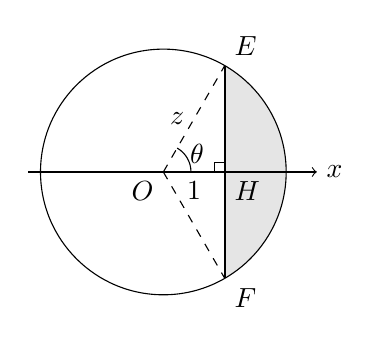
\begin{tikzpicture}[scale=0.78]
                 \fill[gray!20] (1,{-sqrt(3)}) arc[start angle=-60,end angle=60,radius=2] -- cycle;
                 \draw (0,0) circle[radius=2];
                 \draw[thick] (1,{-sqrt(3)}) -- (1,{sqrt(3)});
                 \draw[dashed] (0,0) -- (1,{sqrt(3)}) node[midway,left] {$z$};
                 \draw[dashed] (0,0) -- (1,{-sqrt(3)});
                 \draw[->] (-2.2,0) -- (2.5,0) node[right] {$x$};
                 \draw (0.45,0) arc[start angle=0,end angle=60,radius=0.45];
                 \node at (0.55,0.30) {$\theta$};
                 \node[below left] at (0,0) {$O$};
                 \node[below right] at (1,0) {$H$};
                 \node[above right] at (1,{sqrt(3)}) {$E$};
                 \node[below right] at (1,{-sqrt(3)}) {$F$};
                 \node[below] at (0.5,0) {$1$};
                 \draw (0.84,0) -- (0.84,0.16) -- (1,0.16);
                \end{tikzpicture}
                \end{center}
                図は水平断面で,網掛け部分が求める立体の断面である.
                \,$O$はこの断面の円の中心を表す.
                その面積を$A(z)$とすると,扇形から三角形を引いて,
                \[
                 \begin{aligned}
                 A(z)&=\frac12z^2\cdot2\theta
                      -\frac12\cdot2\sqrt{z^2-1}\cdot1\\
                     &=z^2\theta-\sqrt{z^2-1}.
                 \end{aligned}
                \]
                よって体積は$V=\int_1^2 A(z)\,dz$である.
                \,$z=1/\cos\theta$と置けば,
                \[
                 \sqrt{z^2-1}=\tan\theta,
                 \qquad dz=\frac{\sin\theta}{\cos^2\theta}\,d\theta.
                \]
                したがって,
                \[
                 \begin{aligned}
                 V&=\int_0^{\pi/3}\frac{\theta\sin\theta}{\cos^4\theta}\,d\theta\\
                  &\quad-\int_0^{\pi/3}\frac{\sin^2\theta}{\cos^3\theta}\,d\theta.
                 \end{aligned}
                \]
                第一項では$(\cos^{-3}\theta)'=3\sin\theta/\cos^4\theta$を使って部分積分する.
                第二項では$\sin^2\theta=1-\cos^2\theta$を使うと,
                \[
                 \begin{aligned}
                 V&=\left[\frac{\theta}{3\cos^3\theta}\right]_0^{\pi/3}
                      -\frac13I_3-(I_3-I_1)\\
                  &=\frac{8\pi}{9}-\frac43I_3+I_1\\
                  &=\frac{8\pi}{9}-\frac{4\sqrt3}{3}
                      +\frac13\log(2+\sqrt3).
                 \end{aligned}
                \]
                断面の半径と切断位置の関係を角度で表すと,最初に調べた$I_3$が自然に現れた.
                積分の漸化式は数列だけの技法ではなく,図形から生まれる積分を計算するためにも使える.
          % F6: 一般項を求めずに減衰の速さを決める
          \item 分母に$a_n$があるが,本編の分数型と違って分母が二乗になっている.
                まず逆数を取って,一般項が求められるかだけでなく,増え方を評価できるかを調べる.
                \par\noindent
                \textbf{(1) 逆数の階差を足し合わせる.}
                $a_1=1>0$であり,$a_n>0$なら$(1+2a_n)^2>0$なので$a_{n+1}>0$である.
                よって数学的帰納法からすべての項が正で,$b_n=1/a_n$も定義できる.
                逆数を取ると,
                \[
                 \begin{aligned}
                 b_{n+1}&=\frac{(1+2a_n)^2}{a_n}\\
                         &=b_n+4+4a_n.
                 \end{aligned}
                \]
                したがって$b_{n+1}-b_n=4+4a_n>4$である.
                \,$k=1,\ldots,n-1$について足すと,
                \[
                 b_n-b_1=4(n-1)+4\sum_{k=1}^{n-1}a_k.
                \]
                $b_1=1$より,
                \[
                 b_n=4n-3+4\sum_{k=1}^{n-1}a_k.
                \]
                $n\geq2$なら右辺の総和は正だから,$b_n>4n-3$となる.
                ここまでの変形は,逆数化したあとに階差を総和する本編の技法である.
                ただし総和に$a_k$が残っているため,この式だけでは一般項は得られていない.
                \par\noindent
                \textbf{(2) 項が小さくなることを平均へ移す.}
                正の数の逆数を取ると不等号が逆向きになるので,
                \[
                 0<a_n<\frac1{4n-3}\qquad(n\geq2).
                \]
                挟み撃ちの原理より$a_n\to0$である.
                しかし平均にも$n$が入っているので,項の極限だけで終えず,平均を直接評価する.
                任意の正数$\varepsilon$を取る.
                \,$a_n\to0$より,$k\geq N$なら$0<a_k<\varepsilon$となる正整数$N$が存在する.
                \,$C=\sum_{k=1}^{N-1}a_k$と置けば,$C$は$n$によらない定数である.
                \,$n\geq N$のとき,
                \[
                 \begin{aligned}
                 0<\frac1n\sum_{k=1}^{n}a_k
                 &=\frac Cn+\frac1n\sum_{k=N}^{n}a_k\\
                 &\leq\frac Cn+\frac{n-N+1}{n}\varepsilon\\
                 &\leq\frac Cn+\varepsilon.
                 \end{aligned}
                \]
                十分大きい$n$では$C/n<\varepsilon$でもあるため,平均は$2\varepsilon$より小さい.
                \,$\varepsilon$はいくらでも小さく取れるので,
                \[
                 \lim_{n\to\infty}\frac1n\sum_{k=1}^{n}a_k=0.
                \]
                この証明では,大きかった最初の有限個の項の影響は$n$で割ると消え,
                残りの項はすべて小さい,という二つの点を使っている.
                \par\noindent
                \textbf{(3) 逆数の増え方から元の減衰を読む.}
                (1)の等式を$n$で割ると,
                \[
                 \frac{b_n}{n}=4-\frac3n+
                            \frac4n\sum_{k=1}^{n-1}a_k.
                \]
                (2)より,
                \[
                 0\leq\frac1n\sum_{k=1}^{n-1}a_k
                 \leq\frac1n\sum_{k=1}^{n}a_k\longrightarrow0.
                \]
                したがって$b_n/n\to4$であり,
                \[
                 na_n=\frac1{b_n/n}\longrightarrow\frac14.
                \]
                \par
                最初に求めた上界は,$a_n\to0$を示すための中間結果である.
                それによって階差の追加項$4a_n$の平均が消え,$b_n$は最終的に$4n$と同じ割合で増えると分かった.
                結論$na_n\to1/4$は,$a_n$の減少の速さが$1/(4n)$のそれに近づくことを表す.
                このように,一般項を閉じた式で表さなくても,漸化式から数列の主要な性質を決められる.
          % F7: 1往復で整列できる札の配置
          \item \textbf{(1)~小さい例と, 左端に残る札.}
                $2$枚なら, 昇順の配置はそのまま, 降順の配置は最初の比較で昇順になる.
                よって$c_2=2$である.
                $3$枚では往路の2回の比較で$3$が右端に移る.
                復路では右端の比較は交換を起こさず, 残る2枚が最後の比較で昇順になる.
                したがってすべての配置が成功し,\,$c_3=3!=6$である.
                
                一般に, 最初の比較の直後, 左端の札は
                \[
                  b=\min(A_1,A_2)
                \]
                である. 往路の残りの比較は左端に触れず, 復路でも左端を含む比較は最後に1度だけ行う.
                したがって$b$は最終的に左から1番目か2番目に位置する.
                成功配置ならその数字は$1$または$2$でなければならない.
                これで$\min(A_1,A_2)\le2$が示された.
                ただし, この条件だけで成功が決まるわけではない. 残りの札の並びも調べる必要がある.
                
                \smallskip
                \textbf{(2)~取り除いた札を戻せる対応を作る.}
                比較・交換の結果は, 数字の大小関係だけで決まる.
                そこで札を1枚取り除いた際には, 残りの数字を小さい順に$1,2,\ldots,n-1$と読み替える.
                この読み替えは比較・交換の挙動を変えない.
                
                まず, 成功配置を次の4種類に分ける.
                \[
                \begin{array}{ll}
                \text{\textcircled{1}}&A_1=1,\\
                \text{\textcircled{2}}&A_2=1,\\
                \text{\textcircled{3}}&A_1=2,\ A_2\ge3,\\
                \text{\textcircled{4}}&A_2=2,\ A_1\ge3.
                \end{array}
                \]
                これらは互いに重ならず,\,(1)よりすべての成功配置を尽くす.
                
                \textbf{\textcircled{1},\textcircled{2}の数え方.}
                \textcircled{1}では左端の$1$を取り除く.
                \textcircled{2}では最初の比較によって$1$が左端へ移るので, その$1$を取り除く.
                どちらの場合も, その後の往路は残る$n-1$枚の往路と同じである.
                復路も残る$n-1$枚についての操作を行い, 最後の$1$との比較では交換しない.
                よって元の配置が成功することと, 縮約した配置が成功することは同値である.
                
                逆に,\,$n-1$枚の成功配置の数字をすべて$1$増やし,\,$1$を先頭に挿入すれば\textcircled{1}の配置が得られる.
                $1$を先頭から2番目に挿入すれば\textcircled{2}の配置が得られる.
                いずれも逆操作は一意であるから, 各種類は$c_{n-1}$通りである.
                
                \textbf{\textcircled{3}の数え方.}
                この場合は最初の2枚が$(2,A_2)$で,\,$A_2\ge3$だから最初の比較では交換しない.
                左端の$2$を取り除き, 数字$1$はそのまま,\,$3,4,\ldots,n$をそれぞれ$2,3,\ldots,n-1$に読み替える.
                すると縮約配置の先頭は$1$ではない.
                
                ここで, 元の配置と縮約配置の操作を対応させる.
                元の配置の往路が終わると, 配列は
                \[
                 (2,B_1,B_2,\ldots,B_{n-1})
                \]
                となる. 後ろの$n-1$枚は, 縮約配置の往路後の配列の数字を元に戻したものに等しい.
                復路では, まずこの後ろの$n-1$枚に対し, 縮約問題と同じ比較・交換が行われる.
                
                右から左へ進む1回の操作では, 最小の札$1$は必ずその部分の左端へ移る.
                したがって復路の最後の比較の直前には, 元の配列は
                \[
                 (2,1,D_2,\ldots,D_{n-1})
                \]
                となり, 最後に$(2,1)$が交換される.
                この最終配列が昇順になることは, 縮約問題の最終配列が昇順になることと同値である.
                
                逆に, 先頭が$1$でない$n-1$枚の成功配置で, 数字$2$以上を$1$ずつ増やし,
                先頭に$2$を挿入すれば, 必ず\textcircled{3}の成功配置となる.
                よって求める個数は,\,$n-1$枚の成功配置のうち先頭が$1$でないものの個数である.
                先頭が$1$である成功配置は, 上で示した\textcircled{1}の対応により$c_{n-2}$通りだから,
                \textcircled{3}は$c_{n-1}-c_{n-2}$通りである.
                
                \textbf{\textcircled{4}の数え方.}
                \textcircled{3}の最初の2枚を交換すると,\,$(A_1,2)$で$A_1\ge3$という\textcircled{4}の配置になる.
                最初の比較を済ませれば両者は同じ配列となるので, 成否も一致する.
                この交換は互いに逆だから,\textcircled{4}も$c_{n-1}-c_{n-2}$通りである.
                
                以上を足し合わせると,
                \begin{align*}
                 c_n
                 &=2c_{n-1}+2(c_{n-1}-c_{n-2})\\
                 &=4c_{n-1}-2c_{n-2}\quad(n\ge3).
                \end{align*}
                ここで引いた$c_{n-2}$は, 足し算で生じた曖昧な重複ではなく,
                \textcircled{3}の縮約先から除かなければならない「先頭が$1$の配置」の数である.
                
                \smallskip
                \textbf{(3)~数える問題から, 3項間漸化式へ.}
                特性方程式は
                \[
                 x^2-4x+2=0
                \]
                であり, 根は$2+\sqrt2,2-\sqrt2$である.
                したがって定数$P,Q$を用いて
                \[
                 c_n=P(2+\sqrt2)^{n-1}+Q(2-\sqrt2)^{n-1}
                \]
                と書ける. $c_1=1,c_2=2$より
                \[
                 P+Q=1,\qquad
                 (2+\sqrt2)P+(2-\sqrt2)Q=2.
                \]
                これを解くと$P=Q=1/2$なので,
                \[
                 c_n=\frac{(2+\sqrt2)^{n-1}+(2-\sqrt2)^{n-1}}2.
                \]
                例えば$c_4=20,c_5=68$となる.
                無理数を含む式で配置の個数という整数が表されるのは,
                2つのべきの展開に現れる$\sqrt2$の奇数次の項が相殺されるためである.
                この問題では, 本編の解法を使うまでの「何を数え, 何を取り除くか」の設計が中心である.
          % F8: 巨大な項の整除と, 添字の互除法
          \item \textbf{(1)~余りも漸化式に従う.}
                この数列の最初の項は
                \[
                 1,2,5,26,677,\ldots
                \]
                であり, 値を直接計算して調べ続ける方法はすぐに難しくなる.
                一方,\,$a_n$を$5$で割った余りが$r$なら,
                $a_{n+1}$の余りは$r^2+1$を$5$で割った余りである.
                そこで余りだけを調べると,
                \[
                 1\longmapsto2\longmapsto0\longmapsto1
                \]
                となる. 同じ余りに戻れば, それ以後の余りも同じ規則で繰り返される.
                したがって
                \[
                 a_n\equiv
                 \begin{cases}
                 1 & (n\equiv1\pmod3),\\
                 2 & (n\equiv2\pmod3),\\
                 0 & (n\equiv0\pmod3)
                 \end{cases}
                 \quad(\bmod5).
                \]
                よって$a_n$が$5$の倍数となるのは,\,$n$が$3$の正の倍数であるときに限る.
                
                \smallskip
                \textbf{(2)~法を数列の項にする.}
                補助的に$a_0=0$と定める.
                すると$a_1=a_0^2+1$も成り立つので, 漸化式は$n\ge0$で使える.
                任意の正整数$m$を固定し,
                \[
                 a_{m+j}\equiv a_j\pmod{a_m}
                 \quad(j\ge0)
                \]
                を示そう.
                $j=0$では両辺が$0$と合同である.
                $j$で成り立つと仮定すると,
                \begin{align*}
                 a_{m+j+1}
                 &=a_{m+j}^2+1\\
                 &\equiv a_j^2+1=a_{j+1}\pmod{a_m}.
                \end{align*}
                よって数学的帰納法により, すべての$j\ge0$で成り立つ.
                
                ここで$n=qm+r\ (0\le r<m)$と割り算すると,
                上の合同式を繰り返し使うことで
                \[
                 a_n\equiv a_r\pmod{a_m}
                \]
                が得られる.
                さらに$a_0=0,a_1=1$であり,\,$n\ge1$では
                \[
                 a_{n+1}-a_n=a_n(a_n-1)+1>0
                \]
                だから, 数列は$a_0$から厳密に増加する.
                したがって$0\le r<m$に対して
                \[
                 0\le a_r<a_m,
                \]
                しかも$a_r=0$となるのは$r=0$のときだけである.
                よって
                \begin{align*}
                 a_m\mid a_n
                 &\Longleftrightarrow a_r=0\\
                 &\Longleftrightarrow r=0\\
                 &\Longleftrightarrow m\mid n.
                \end{align*}
                この議論は$m=1$でも成り立つ. このとき余りの添字は必ず$r=0$で,
                $a_1=1$はすべての整数を割り切る.
                なお,\,$a_3=5$であるから,\,(1)はこの結果の$m=3$という特別な場合でもある.
                
                \smallskip
                \textbf{(3)~項の互除法を, 添字の互除法へ移す.}
                再び$n=qm+r\ (0\le r<m)$とおく.
                $a_n\equiv a_r\pmod{a_m}$であるから,\,$a_n$と$a_r$の差は$a_m$の整数倍である.
                よって$a_m$と$a_n$の共通の約数は,\,$a_m$と$a_r$の共通の約数に一致する.
                したがって
                \[
                 \gcd(a_m,a_n)=\gcd(a_m,a_r).
                \]
                これは, 添字に対して行うユークリッドの互除法に沿って,
                項の最大公約数を保ったまま添字を小さくできることを意味する.
                添字の互除法は,\,$d=\gcd(m,n)$と$0$で終わるので,
                \[
                 \gcd(a_m,a_n)=\gcd(a_d,a_0)=a_d.
                \]
                最後の等号は,\,$a_0=0$であり,\,$\gcd(x,0)=x$だからである.
                
                求める例では,
                \begin{align*}
                 3040&=2026+1014,\\
                 2026&=1014+1012,\\
                 1014&=1012+2,\\
                 1012&=506\cdot2
                \end{align*}
                だから,\,$\gcd(2026,3040)=2$である.
                従って
                \[
                 \gcd(a_{2026},a_{3040})=a_2=2.
                \]
                項がどれほど大きくなっても, 添字の小さな整数計算だけでこの最大公約数が決まる.
                漸化式は項の値を求めるだけでなく, 整除のような「項どうしの関係」を取り出す道具にもなる.
          % F9: 整数方程式の解を生み出す漸化式
          \item \textbf{(1)~1つの解から次の解へ.}
                $x=3$のとき, 方程式は
                \[
                 9+y^2+z^2=3yz
                \]
                となる. $z$を固定して$y$の2次方程式とみれば,
                もう1つの根は$3z-y$であることが, 根と係数の関係から予想できる.
                実際に確かめると,
                \begin{align*}
                 &9+z^2+(3z-y)^2-3z(3z-y)\\
                 &\qquad=9+y^2+z^2-3yz=0.
                \end{align*}
                よって$(3,z,3z-y)$も方程式を満たす.
                しかも$3z-y$は整数であり,\,$0<y\le z$より
                \[
                 3z-y\ge2z>z>0.
                \]
                したがって正の整数解である.
                この操作で新しくできた2つの数も$z<3z-y$を満たすため, 同じ操作を繰り返せる.
                
                \smallskip
                \textbf{(2)~解を作る操作を数列にする.}
                最初の解$(3,3,3)$から(1)の操作を繰り返すと,\,$y,z$は
                \[
                 (3,3),\ (3,6),\ (6,15),\ (15,39),\ldots
                \]
                と変化する.
                この隣接する2つの数を$u_n,u_{n+1}$とすれば, 次の数は$3u_{n+1}-u_n$となる.
                これが問題で与えた3項間漸化式の意味である.
                
                特性方程式は
                \[
                 t^2-3t+1=0
                \]
                であり, 2つの根を
                \[
                 \alpha=\frac{3+\sqrt5}2,\qquad
                 \beta=\frac{3-\sqrt5}2
                \]
                とおく.
                $u_n=P\alpha^n+Q\beta^n$と書くと,\,$u_0=u_1=3$より
                \[
                 P+Q=3,\qquad \alpha P+\beta Q=3.
                \]
                これを解けば
                \[
                 P=\frac{3(\sqrt5-1)}{2\sqrt5},\qquad
                 Q=\frac{3(\sqrt5+1)}{2\sqrt5}.
                \]
                したがって
                \begin{align*}
                 u_n
                 &=P\alpha^n+Q\beta^n\\
                 &=\frac32\left\{\alpha^n+\beta^n
                 -\frac{\alpha^n-\beta^n}{\sqrt5}\right\}.
                \end{align*}
                
                \smallskip
                \textbf{(3)~一般項とは別に, 整数性と方程式を保証する.}
                初期値は整数であり, 漸化式は整数の3倍と整数の差で次の項を作る.
                したがって数学的帰納法により, すべての$u_n$は整数である.
                また$u_0=u_1=3>0,u_2=6>u_1$である.
                $u_{n+1}>u_n>0$なら
                \[
                 u_{n+2}=3u_{n+1}-u_n>2u_{n+1}>u_{n+1}
                \]
                だから,\,$n\ge1$で$u_{n+1}>u_n>0$が成り立つ.
                
                さらに, 隣接する2項から作る量
                \[
                 I_n=u_n^2+u_{n+1}^2-3u_nu_{n+1}
                \]
                を考える.
                漸化式を代入すると,
                \begin{align*}
                 I_{n+1}
                 &=u_{n+1}^2+(3u_{n+1}-u_n)^2\\
                 &\quad{}-3u_{n+1}(3u_{n+1}-u_n)\\
                 &=u_n^2+u_{n+1}^2-3u_nu_{n+1}=I_n.
                \end{align*}
                従ってこの量は変わらず,
                \[
                 I_n=I_0=9+9-27=-9.
                \]
                よって
                \[
                 3^2+u_n^2+u_{n+1}^2=3u_nu_{n+1}.
                \]
                以上から$(3,u_n,u_{n+1})$は正の整数解である.
                $n\ge1$で$u_{n+1}$が厳密に増加するので, これらの三つ組は互いに異なり, 解は無限個ある.
                ここでは特定の操作で得られる解の系列を作っており, すべての解の分類までは要求していない.
                
                最後に比の極限を求める.
                $0<\beta<1<\alpha$であり,\,$P,Q>0$だから,
                \[
                 \frac{u_{n+1}}{u_n}
                 =\alpha\,
                 \frac{P+Q(\beta/\alpha)^{n+1}}
                      {P+Q(\beta/\alpha)^n}
                 \longrightarrow\alpha.
                \]
                一般項には無理数が現れるが, 漸化式が整数性を保証する.
                さらに整数どうしの比が無理数$\alpha$へ近づくことまで分かる.
                解法としての3項間漸化式が, 整数解を無限に生成する仕組みと, その増加の速さを同時に記述している.
          % F10: 元のペアをすべて解消する組み替え
          \item \textbf{(1) 小さい場合で数える対象を確認する.}
                $n=1$では組み替える相手がいないため,\,$S(1)=0$である.
                $n=2$では$(A_1,B_2),(A_2,B_1)$の1通りである.
                $n=3$では,\,$A_1,A_2,A_3$の相手の添字が
                $(2,3,1)$または$(3,1,2)$となる2通りなので,\,$S(3)=2$である.
                $S(0)=1$は, 要素がない場合の「何も作らない組合せ」を1通りと数える約束である.
                \par\smallskip
                \textbf{(2) 相手を1個決め, 残りを小さい問題に戻す.}
                $A_1$の相手$B_j$は,\,$j\ne1$の$n-1$通りから選ぶ.
                以後は$j$を固定する.
                \par
                まず$A_j$の相手が$B_1$なら,\,$A_1,A_j,B_1,B_j$を除いた残りの$n-2$組を,
                元のペアが残らないように作ればよい.
                これは$S(n-2)$通りである.
                \par
                次に$A_j$の相手が$B_1$でないとする.
                $B_1$の相手を$A_k$とすると,\,$k\ne1,j$である.
                2組のペア
                \[
                 (A_1,B_j),\quad(A_k,B_1)
                \]
                から$A_1,B_1$を除き,\,$(A_k,B_j)$の1組に置き換える.
                $k\ne j$なので, この新しいペアも元のペアではない.
                したがって, 添字$2,\ldots,n$の$n-1$組を完全に組み替えた形になる.
                \par
                逆に, そのような$n-1$組の組合せから$B_j$の相手$A_k$を見つけ,
                \[
                 (A_k,B_j)\ \longmapsto
                 (A_1,B_j),(A_k,B_1)
                \]
                と戻せば, 元の組合せが一意に復元できる.
                つまり, 対応は一対一であり, 後者は$S(n-1)$通りである.
                この「小さくした問題に戻せること」が, 個数の漸化式を作る根拠である.
                2つの場合は重ならないので,
                \[
                 S(n)=(n-1)\{S(n-1)+S(n-2)\}.
                \]
                \par\smallskip
                \textbf{(3) 変動する係数を, 差と階乗で整理する.}
                この漸化式は係数が$n$に依存するため, 定数係数の3項間漸化式としては解けない.
                そこで
                \[
                 T_n=S(n)-nS(n-1)\quad(n\ge1)
                \]
                とおく. $n\ge2$では(2)から
                \begin{align*}
                 T_n
                 &= (n-1)S(n-2)-S(n-1)\\
                 &= -T_{n-1}.
                \end{align*}
                $T_1=S(1)-S(0)=-1$より,\,$T_n=(-1)^n$である.
                よって
                \[
                 S(n)=nS(n-1)+(-1)^n.
                \]
                ここで$n$を階比として吸収するため,\,$P_n=S(n)/n!$とおく.
                \[
                 P_n-P_{n-1}=\frac{(-1)^n}{n!}.
                \]
                $P_0=S(0)/0!=1$より, 階差を足し合わせると
                \[
                 P_n=\sum_{k=0}^{n}\frac{(-1)^k}{k!}.
                \]
                したがって,
                \[
                 S(n)=n!\sum_{k=0}^{n}\frac{(-1)^k}{k!}.
                \]
                なお,\,$S(4)=9,\,S(5)=44$もこの式や(2)から求められる.
                本編の\textbf{等比型, 階比による正規化, 階差型}を順に使ったことになる.
                \par\smallskip
                \textbf{(4) 残る組数を指定して数える.}
                元のペアをちょうど$r$組残すには, まず残す$r$組を$\binom{n}{r}$通りから選ぶ.
                残りの$n-r$組では元のペアを1組も残せないので, その組み方は$S(n-r)$通りである.
                どの$r$組が残るかは完成形から一意に決まるため, 重複はない.
                よって答えは
                \[
                 \binom{n}{r}S(n-r)
                \]
                である. $r=n$でも$S(0)=1$によって1通りと数えられる.
                \par
                次に, 全組合せで残る元のペアの組数を合計する.
                固定したペア$(A_i,B_i)$が残る組合せは, 残りの相手を自由に割り当てる$(n-1)!$通りである.
                これを$i=1,\ldots,n$について足すと, 合計は$n(n-1)!$となる.
                元のペアが$r$組残る組合せはちょうど$r$回数えられるので, この合計でよい.
                全組合せは$n!$通りであるから, 平均値は$n(n-1)!/n!=1$である.
                \par\smallskip
                \noindent\textbf{【数学的な広がり：完全順列と確率】}\par\nopagebreak[4]
                元の位置に戻る要素のない並べ替えを\textbf{完全順列（錯置）}と呼ぶ.
                この問題はその数え上げである.
                また, 全$n!$通りを同じ確率で選ぶとき, 元のペアが1組も残らない確率は
                \[
                 P_n=\frac{S(n)}{n!}
                     =\sum_{k=0}^{n}\frac{(-1)^k}{k!}
                \]
                である. このように,\,$n!$で割る操作には, 漸化式を整理するだけでなく\textbf{個数を確率に直す意味}もある.
                \par
                さらに, この確率は$n$が大きくなると$1/e$に近づく.
                ここでは無限級数展開を仮定せず, 本編の二項定理と$e$の定義で確認しよう.
                \par
                まず$m\ge0$について,
                \begin{align*}
                 P_{2m+2}-P_{2m}
                 &= -\frac{2m+1}{(2m+2)!}<0,\\
                 P_{2m+3}-P_{2m+1}
                 &= \frac{2m+2}{(2m+3)!}>0.
                \end{align*}
                また,\,$P_{2m}-P_{2m+1}=1/(2m+1)!$である.
                したがって, 偶数番目の確率は減少し, 奇数番目の確率は増加し, 両者の差は0へ近づく.
                確率は$0$以上$1$以下なので, それぞれ収束し, 共通の極限$L$をもつ.
                \par
                その値を決めるため, 整数$M\ge2$に対して
                \[
                 b_{M,k}=\frac{\binom{M}{k}}{M^k}
                 \quad(0\le k\le M)
                \]
                とおく. すると
                \[
                 \frac{b_{M,k+1}}{b_{M,k}}
                 =\frac{M-k}{M(k+1)}\le1
                \]
                なので,\,$b_{M,k}$は$k$について非増加である.
                二項定理の有限和を,添字$k$が偶数または奇数の項で止める.
                残りを隣り合う2項ずつ組にすることで,
                $M\ge2\ell+1$に対して
                \begin{align*}
                 \sum_{k=0}^{2\ell+1}(-1)^k b_{M,k}
                 &\le\left(1-\frac1M\right)^M,\\
                 \left(1-\frac1M\right)^M
                 &\le\sum_{k=0}^{2\ell}(-1)^k b_{M,k}
                \end{align*}
                が分かる. 添字が奇数の項で止めた残りは「正の項$-$次の項」の和となり0以上で,
                添字が偶数の項で止めた残りはその符号が逆になる.
                \par
                ここで$\ell$を固定し,\,$M\to\infty$とする.
                固定した$k$について
                \[
                 b_{M,k}=\frac1{k!}
                 \prod_{j=0}^{k-1}\left(1-\frac jM\right)
                 \longrightarrow\frac1{k!}.
                \]
                $k=0$の積は$1$とする.
                一方,\,$t=M-1$とおくと,
                \[
                 \left(1-\frac1M\right)^M
                 =\left(1+\frac1t\right)^{-t-1}.
                \]
                本編の$e$の定義から,$(1+1/t)^t\to e$であり,
                $(1+1/t)\to1$なので,上の式は$1/e$へ近づく.
                よって
                \[
                 P_{2\ell+1}\le\frac1e\le P_{2\ell}.
                \]
                今度は$\ell\to\infty$とし, 挟み撃ちによって$L=1/e$を得る.
                \[
                 \boxed{\lim_{n\to\infty}\frac{S(n)}{n!}
                       =\frac1e\simeq0.368}.
                \]
                同じ偶奇の後の項は極限へ向かって厳密に進むため,
                $1/e$は隣り合う$P_n,P_{n+1}$の間に厳密に入る. よって$n\ge1$で
                \begin{align*}
                 \left|P_n-\frac1e\right|
                 &<\frac1{(n+1)!},\\
                 \left|S(n)-\frac{n!}{e}\right|
                 &<\frac1{n+1}\le\frac12.
                \end{align*}
                下段は上段を$n!$倍して得られる.
                つまり,\,$S(n)$は$n!/e$に最も近い整数である.
                場合の数を数える漸化式から, 階乗, 確率, 自然対数の底が一つにつながった.
        \end{enumerate}

